%%%%%%%%%%%%%%%%%%%%%%%%%%%%%%%%%%%%%%%%%%%%%%%%%%%%%%%%%%%%%%%%%%%%%%%%%%%%%%%%%%%%%%%
%%%%%%%%%%%%%%%%%%%%%%%%%%%%%%%%%%%%%%%%%%%%%%%%%%%%%%%%%%%%%%%%%%%%%%%%%%%%%%%%%%%%%%%
% 
% This top part of the document is called the 'preamble'.  Modify it with caution!
%
% The real document starts below where it says 'The main document starts here'.

\documentclass[12pt]{article}

\usepackage{amssymb,amsmath,amsthm}
\usepackage[top=1in, bottom=1in, left=1.25in, right=1.25in]{geometry}
\usepackage{fancyhdr}
\usepackage{enumerate}
\usepackage{graphicx}
\usepackage{gensymb}
\usepackage{soul}
\usepackage{pdfpages}
% Comment the following line to use TeX's default font of Computer Modern.
\usepackage{times,txfonts}

\newtheoremstyle{homework}% name of the style to be used
  {18pt}% measure of space to leave above the theorem. E.g.: 3pt
  {12pt}% measure of space to leave below the theorem. E.g.: 3pt
  {}% name of font to use in the body of the theorem
  {}% measure of space to indent
  {\bfseries}% name of head font
  {:}% punctuation between head and body
  {2ex}% space after theorem head; " " = normal interword space
  {}% Manually specify head
\theoremstyle{homework} 

% Set up an Exercise environment and a Solution label.
\newtheorem*{exercisecore}{Exercise \@currentlabel}
\newenvironment{exercise}[1]
{\def\@currentlabel{#1}\exercisecore}
{\endexercisecore}

\newcommand{\localhead}[1]{\par\smallskip\noindent\textbf{#1}\nobreak\\}%
\newcommand\solution{\localhead{Solution:}}

%%%%%%%%%%%%%%%%%%%%%%%%%%%%%%%%%%%%%%%%%%%%%%%%%%%%%%%%%%%%%%%%%%%%%%%%
%
% Stuff for getting the name/document date/title across the header
\makeatletter
\RequirePackage{fancyhdr}
\pagestyle{fancy}
\fancyfoot[C]{\ifnum \value{page} > 1\relax\thepage\fi}
\fancyhead[L]{\ifx\@doclabel\@empty\else\@doclabel\fi}
\fancyhead[C]{\ifx\@docdate\@empty\else\@docdate\fi}
\fancyhead[R]{\ifx\@docauthor\@empty\else\@docauthor\fi}
\headheight 15pt

\usepackage{listings}
\usepackage{color}

\definecolor{dkgreen}{rgb}{0,0.6,0}
\definecolor{gray}{rgb}{0.5,0.5,0.5}
\definecolor{mauve}{rgb}{0.58,0,0.82}


\def\doclabel#1{\gdef\@doclabel{#1}}
\doclabel{Use {\tt\textbackslash doclabel\{MY LABEL\}}.}
\def\docdate#1{\gdef\@docdate{#1}}
\docdate{Use {\tt\textbackslash docdate\{MY DATE\}}.}
\def\docauthor#1{\gdef\@docauthor{#1}}
\docauthor{Use {\tt\textbackslash docauthor\{MY NAME\}}.}
\makeatother

% Shortcuts for blackboard bold number sets (reals, integers, etc.)
\newcommand{\Reals}{\ensuremath{\mathbb R}}
\newcommand{\Nats}{\ensuremath{\mathbb N}}
\newcommand{\Ints}{\ensuremath{\mathbb Z}}
\newcommand{\Rats}{\ensuremath{\mathbb Q}}
\newcommand{\Cplx}{\ensuremath{\mathbb C}}
%% Some equivalents that some people may prefer.
\let\RR\Reals
\let\NN\Nats
\let\II\Ints
\let\CC\Cplx

%%%%%%%%%%%%%%%%%%%%%%%%%%%%%%%%%%%%%%%%%%%%%%%%%%%%%%%%%%%%%%%%%%%%%%%%%%%%%%%%%%%%%%%
%%%%%%%%%%%%%%%%%%%%%%%%%%%%%%%%%%%%%%%%%%%%%%%%%%%%%%%%%%%%%%%%%%%%%%%%%%%%%%%%%%%%%%%
% 
% The main document start here.

% The following commands set up the material that appears in the header.
\doclabel{Stat 300: Homework 1}
\docauthor{Stefano Fochesatto}
\docdate{\today}

\begin{document}





\begin{exercise}{1.14} The accompanying data set consists of observations on shower-flow rate for a sample of $n = 129$ houses in Perth, Australia.
  \begin{enumerate}
    \item[\textbf{a.}] Construct a stem-and-leaf display of the data.\\
    \textbf{Solution:}
    \begin{lstlisting}
      > stem(x)

      The decimal point is at the |
    
       2 | 23
       3 | 2344567789
       4 | 01356889
       5 | 00001114455666789
       6 | 0000122223344456667789999
       7 | 00012233455555668
       8 | 02233448
       9 | 012233335666788
      10 | 2344455688
      11 | 2335999
      12 | 37
      13 | 8
      14 | 36
      15 | 0035
      16 | 
      17 | 
      18 | 9    
    \end{lstlisting}

    \vspace{.5in}
     
    \item[\textbf{b.}] What is a typical, or representative flow rate?\\
    
    \textbf{Solution:}
    
    \begin{lstlisting}
    > fivenum(x)
 Minimum   Lower Quartile  Median  Upper Quartile  Maximum 
     2.2        5.6        7.0        9.6       18.9 
      
    > mean(x)
      [1] 7.707752
  
    > sd(x)
      [1] 3.076844
    \end{lstlisting}
    I would say that a representative flow rate would be closer to the median at $7.0$ since there is an outlier in $18.9$ that is more than 3 standard deviations away from the mean.
    \vspace{.5in}
     
    \item[\textbf{c.}] Does the display appear to be highly concentrated or spread out?\\
    
    \textbf{Solution:} Generally speaking this display appears to be highly concentrated with a small slight skew towards the right.
    \vspace{.5in}
     

    \item[\textbf{d}] Does the distribution of values appear to be reasonably symmetric?If not, how would you describe the departure from symmetry?\\
    
    \textbf{Solution:} The data is does not appear to be symmetrical, since it seems to have a slight positive skew.
    \vspace{.5in}


    \item[\textbf{e}] Would you describe any observation as being far from the rest of the data (an outlier)?\\
    
    \textbf{Solution:} I would describe the data point $x = 18.9$ as an outlier, since it is almost 4 standard deviations from the mean.  
    \vspace{.5in}
     

  \end{enumerate}
\end{exercise}
\vspace{1in}



\begin{exercise}{1.18} Every corporation has a governing board og directors. The number of individuals on a board varies from one corporation to another. One of the authors of the article provided the accompanying data on the number of directors on each board in a random sample of 204 corporations.\\
  \begin{enumerate}
    \item[\textbf{a.}] Construct a histogram of the data based on relative frequencies and comment on any interesting features?\\
    
    \textbf{Solution:}
    \begin{center}
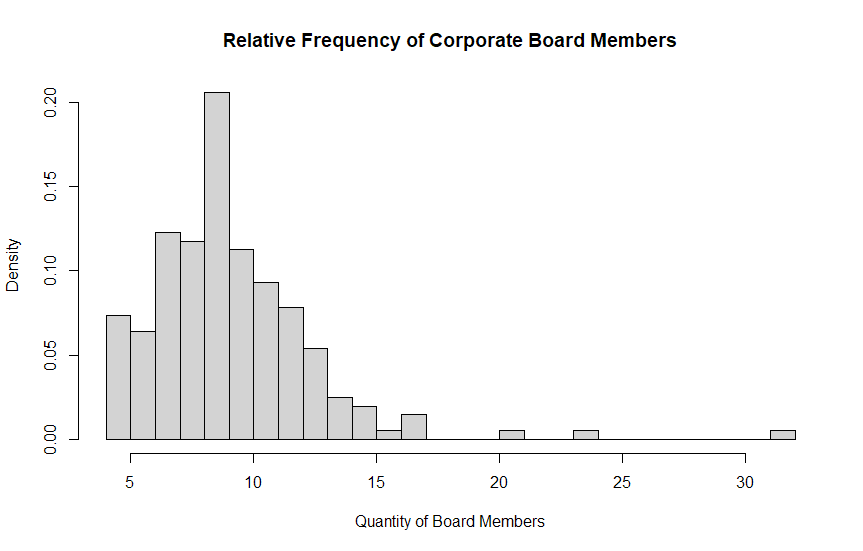
\includegraphics[width=\textwidth]{hist.png}      
    \end{center}
    The distribution appears to be roughly unimodal and right skewed. The data set contains outliers at (21,24,32) as there are gaps in the histogram. Spread appears to be between 4 to 17 with a majority of corporations having 9 members. 

    \vspace{.5in}
     
    \item[\textbf{c.}] What proportion of these corporations have at most 10 directors.\\
    
    \textbf{Solution:}

    \begin{lstlisting}
    > View(ex01.18)
    > x = X.Frequenc.
    > sum(x)
      [1] 204
    > sum = 0;
    % 7 = Index of the value of 10
    > for (i in 1:7){
      +   sum<- sum+x[i]
      + }
    > sum
      [1] 142
    > 142/204
      [1] 0.6960784
    \end{lstlisting}
    Thus the proportion of companies with at most 10 board members is $\frac{142}{204} \approx .6961$ or 69.61\%. 
    
    \vspace{.5in}
     
  \end{enumerate}


\end{exercise}
\vspace{1in}


\begin{exercise}{1.22} How does the speed of a runner vary over the course of a marathon? Consider determining both the time to run the first 5km and 
  the run between the 35-km and 40-km points, and then subtracting the former time from the latter time. A positive value of this difference corresponds to a runner slowing down toward the end of the race.
  The accompanying histogram is based on times of runners who participated in several different Japanese marathons. What are some interesting features of this histogram?
  What is a typical difference value? Roughly what proportion of runners ran the late distance more quickly than the early distance?\\
  \begin{center}
    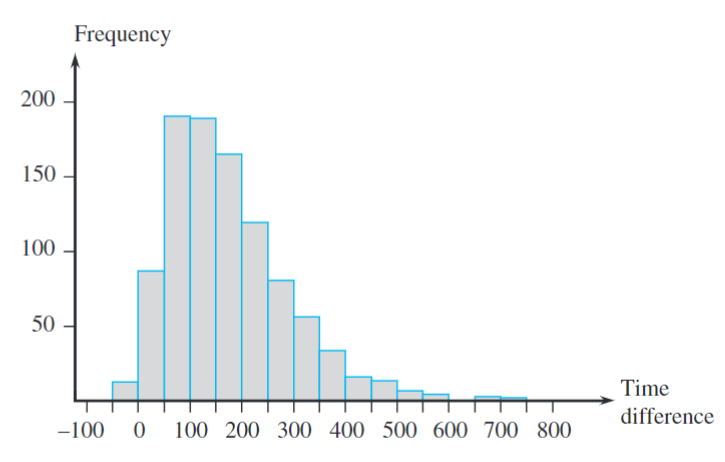
\includegraphics[width=\textwidth]{hist2.png}      
  \end{center}
  
  \textbf{Solution:}
  Again this histogram appears to be roughly unimodal with a noticeable right skew. Since a positive value of the difference means that the runner is slowing down 
  at the end of the race the histogram shows us that a large majority of runners are in fact slowing down. Furthermore since the histogram is positively skewed we know that
  some runners seem to slow down much more than the median runner, making the average greater and creating a positive skew. Given that the histogram is unimodal we can hazard a guess that the 
  representative value would be around 175 seconds. Roughly estimating the proportion of runners ran the late distance more quickly than the early distance I would say they account for less than 1\% of the population.

\end{exercise}
\vspace{1in}



\begin{exercise}{1.38} Blood pressure values are often reported to the nearest 5 mmHg. Suppose the actual blood pressure values for nine randomly selected individuals are,

\begin{lstlisting}
'Blood_Pres (mmHg)'
118.599998474121
127.400001525879
138.399993896484
130
113.699996948242
122
108.300003051758
131.5
133.199996948242
\end{lstlisting}
\begin{enumerate}
  \item[\textbf{a.}] What is the median (and mean) of the reported blood pressure values?\\
  
  \textbf{Solution:}
  \begin{lstlisting}
  >   View(ex01.38)
  > x <- ex01.38$X.Blood_Pres
  > fivenum(x)
  Minimum   Lower Quartile  Median  Upper Quartile  Maximum 
  108.3       118.6        127.4        131.5       138.4 
  > mean(x)
    [1] 124.7889
\end{lstlisting}
From the $r$ computation we can see that the $Median = 127.4$ and the $Mean = 124.788$. 
  \vspace{.5in}

  
  
  
  \item[\textbf{b.}]Suppose the blood pressure of the second individual is 127.6 rather than 127.4. How does this affect the median of the reported values?
  What does this say about the sensitivity of the median to rounding or grouping in the data?\\
  
  [\textbf{Solution:}]
  
  \begin{lstlisting}
  > x[2] = 127.6
  > fivenum(x)
  Minimum   Lower Quartile  Median  Upper Quartile  Maximum 
  108.3       118.6        127.6        131.5       138.4 
  > mean(x)
    [1] 124.8111
  \end{lstlisting}
  We can see that our rounding experiment a greater effect on the median than the mean with a $\delta$ of .2 as apposed to a $\delta$ of .03. 
  Had our rounding been enough to change the order of our data points I could see it greatly affecting the median, however in this case it did not. Note 
  that the median is not sensitive to the grouping of data since by definition it is simply the middle value. For example suppose a bimodal data set where the median occurs at the trough.
\end{enumerate}

\end{exercise}
\vspace{1in}


\begin{exercise}{1.42}                                                                                                               
  \hfill \break
  \begin{enumerate}
  \item[\textbf{a.}] If a constant $c$ is added to each $x_i$ in a sample, yielding $y_i = x_i + c$, how do the sample mean and median of the $y_{i}s$
  relate to the mean and median of the $x_{i}s$? Verify you conjectures. \\
 
  \textbf{Proof:} Suppose a sample set $y$ and $x$ such that $y_i = x_i + c$. By the definition of sample mean we know,
  \begin{equation*}
    \overline{y}= \frac{\sum_{i = 1}^{n} y_i}{n}.
  \end{equation*}
  \vspace{.5in}
  Using our definition of $y_i$ and some algebra we get,
  \begin{align*}
    \overline{y} &= \frac{\sum_{i = 1}^{n} x_i + c}{n},\\
    &= \frac{(\sum_{i = 1}^{n} x_i)+(cn)}{n},\\
    &= \overline{x} + c.
  \end{align*}
  Thus we have shown that the given sample results in a sample mean of $\overline{y} = \overline{x} + c$. Furthermore, regardless of the parity of $n$, the middle value, and average of the two middle values 
  still gets shifted by $c$ therefore we get that $\hat{y} = \hat{x} + c$.\\
  \qed

  \item[\textbf{b.}] If each $x_i$ is multiplied by a constant $c$, yielding $y_i = cx_i$, answer the questions of part $a$. Again verify you conjectures.\\
  
  \textbf{Proof:} Similarly suppose a sample set $y$ and $x$ such that $y_i = cx_i$. By the definition of sample mean we know,
  \begin{equation*}
    \overline{y}= \frac{\sum_{i = 1}^{n} y_i}{n}.
  \end{equation*}
  \vspace{.5in}
  Using our definition of $y_i$ and some algebra we get,
  \begin{align*}
    \overline{y} &= \frac{\sum_{i = 1}^{n} cx_i}{n},\\
    &= \frac{(c\sum_{i = 1}^{n} x_i)}{n},\\
    &= c\overline{x}.
  \end{align*}
  We have shown that the given sample results in a sample mean of $\overline{y} = c\overline{x}$. And again, regardless of the parity of $n$, the middle value, and average of the two middle values 
  still gets shifted by $c$ therefore we get that $\hat{y} = c\hat{x}$.\\
  \qed
\end{enumerate}

\end{exercise}
\vspace{1in}





\begin{exercise}{1.44} Poly (3-hydroxybutyrate) (PHB), a semicrystalline polymer that is fully biodegradable and bio-compatible,
  is obtained from renewable resources. From a sustainability perspective, PHB offers many attractive properties though it is more expensive
  to produce than standard plastics. The accompanying data on melting point ($\degree C$) for each 12 specimens of the polymer using a differential scanning
  calorimeter. 
\begin{enumerate}
  \item[\textbf{a.}] Compute the sample range.\\
  
  \textbf{Solution:} 
  \begin{lstlisting}
    >   View(ex01.44)
    > x <- ex01.44$X.Melting_Point.
    > max(x)-min(x)
      [1] 2.3
  \end{lstlisting}
  Therefore the sample range is 2.3 $\degree C$.
  \vspace{.5in}


  \item[\textbf{b.}] Compute the sample variance $s^2$ from the definition. [Hint: First subtract 180 from each observation.]\\
  
  \textbf{Solution:}
  Recall the definition of $s^2$,
  \begin{equation*}
    s^2 = \sum_{i = 1}^n (x_i - \overline{x})^2 \cdot \frac{1}{n-1}.
  \end{equation*}
  From the r computation,
  \begin{lstlisting}
  > x <- ex01.44$X.Melting_Point.
  > m = mean(x)
  > y = x-m
  > sum(y^2)/11
    [1] 0.5244697
  \end{lstlisting}
  we get that the sample variance, $s^2 = 0.5244697$.
  \vspace{.5in}


  \item[\textbf{c.}] Compute the sample standard deviation $s$ .\\
  
  \textbf{Solution:}
  By the definition of sample standard deviation we know that it is simply the positive square root of the sample variance. Thus $s = 0.7242028$
   
\end{enumerate}
\end{exercise}
\vspace{1in}







\begin{exercise}{1.50} In 1997 a woman sued a computer keyboard manufacturer, charging that her repetitive stress injuries were caused by the keyboard.
  The injury awarded about 3.5 million for pain and suffering, but the court then set aside that award as being unreasonable compensation. In making this 
  determination, the court identifies a "normative" group of 27 similar cases and specifies a reasonable award as one within two standard deviations of the mean of the awards in the 27 cases.
  What is the maximum possible amount that could be awarded under the two-standard-deviation rule?\\
  
  \textbf{Solution:} 
  \begin{lstlisting}
    > x <- ex01.50$X.awards.
    > m = mean(x)
    > ss = sd(x)
    > m+2*ss
      [1] 1961.158
  \end{lstlisting}
  The maximum amount that could be awarded under the 2-standard-deviation rule is \$1,961,158. Any more would not be within 2 standard deviations.
\end{exercise}
\vspace{1in}









\begin{exercise}{1.56} The following data on distilled alcohol content for a sample of 35 port wines. Each value is an average of two duplicate measurements.
  Use methods from this chapter, including a boxplot that show outliers, to describe and summarize the data.\\

  \textbf{Solution:}
  Analyzing the data with r,
  \begin{lstlisting}
    > x <- ex01.56$X.alcohol
    > fivenum(x)
    Minimum   Lower Quartile  Median  Upper Quartile  Maximum 
    15.30       18.34        19.20        19.76       23.78 
    > mean(x)
      [1] 19.25743
    > sd(x)
      [1] 1.831662
    > var(x)
      [1] 3.354984
    > IQR(x)
      [1] 1.42
    > boxplot(x, horizontal = TRUE, ylab = 'Port Wines',
      +         xlab = 'Distilled Alcohol Content (%)', col = "orange",
      +         border = "brown", notch = TRUE)
  \end{lstlisting}
  \begin{center}
    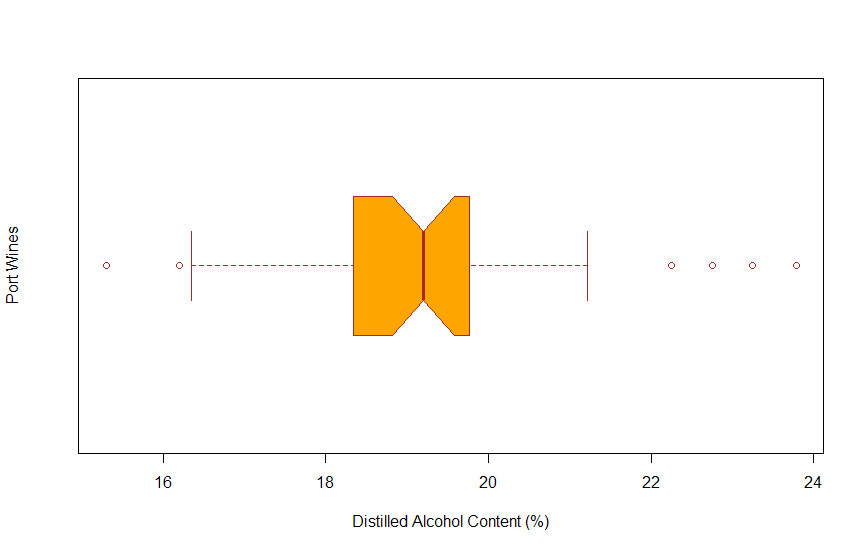
\includegraphics[width=\textwidth]{Boxplot.png}      
  \end{center}
  Firstly we can see that there is a relatively small $\delta$ between the upper/lower forth and the median, the relatively small IQR and the $\delta$ between the median and the mean, 
  despite the large number of positive outliers demonstrated in the
  boxplot suggests that most of the data points are grouped between 18 to 20 percent. Furthermore this means that the representative value could be either the mean or median.






\end{exercise}
\vspace{1in}



\begin{exercise}{2.4} Each of a sample of four home mortgages is classifies as fixed rate (F) or variable rate (V).\\

  \begin{enumerate}
    \item[\textbf{a.}] What are the 16 outcomes of $s$\\

    \textbf{Solution:}
    \begin{equation*}
    s = \begin{bmatrix}
      FFFF & VFFF & FVFV & VVFV\\
      FFFV & FFVV & VFFV & VFVV\\
      FFVF & FVVF & VFVF & FVVV\\
      FVFF & VVFF & VVVF & VVVV
    \end{bmatrix}
    \end{equation*}
    \vspace{.5in}

    
    
    
    
    \item[\textbf{b.}] Which outcomes are in the event that exactly three of the selected mortgages are fixed?\\
    
    \textbf{Solution:} 
    \begin{equation*}
     \begin{bmatrix}
        VFFF \\
        FFFV \\
        FFVF \\
        FVFF 
      \end{bmatrix}
      \end{equation*}
    \vspace{.5in}
    
    
    
    
    
    \item[\textbf{c.}] Which outcomes are in the event that all four mortgages are of the same type?\\
     
    \textbf{Solution:}
    \begin{equation*}
      \begin{bmatrix}
        FFFF \\
        VVVV
    \end{bmatrix}
    \end{equation*}
    \vspace{.5in}
    
    
    
    
    
    \item[\textbf{d.}] Which outcomes are in the event that at most one of the four is a variable-rate mortgage?\\
    
    \textbf{Solution:}
    \begin{equation*}
      \begin{bmatrix}
        FFFF \\
        FFFV \\
        FFVF \\ 
        FVFF \\
        VFFF 
      \end{bmatrix}
      \end{equation*}

    \vspace{.5in}
    
    
    
    
    \item[\textbf{e.}] What is the union of the events in parts (c) and (d), and what is the intersection of these two events?\\
     
    \textbf{Solution:}
    \begin{equation*}
      c \cup d =       
      \begin{bmatrix}
        VFFF \\
        FFFV \\
        FFVF \\
        FVFF 
      \end{bmatrix}
      \end{equation*}

      \begin{equation*}
        c \cap d =       
        \begin{bmatrix}
          FFFF 
        \end{bmatrix}
        \end{equation*}
    \vspace{.5in}
    
    
    
    \item[\textbf{f.}] What is the union of the events in parts (c) and (b), and what is the intersection of these two events?\\
     
    
    \textbf{Solution:}
    \begin{equation*}
      c \cup b =       
      \begin{bmatrix}
        VVVV \\
        FFFF \\
        FFFV \\
        FFVF \\ 
        FVFF \\
        VFFF 
      \end{bmatrix}
      \end{equation*}

      \begin{equation*}
        c \cap b = \varnothing
        \end{equation*}

  \end{enumerate}
\end{exercise}
\vspace{1in}




\begin{exercise}{2.9} Use Venn Diagrams to verify the following two relationships for any events $A$ and $B$,
  \begin{enumerate}
    \item[\textbf{a.}] $(A \cap B)' = A' \cup B'$ 
    \item[\textbf{b.}] $(A \cup B)' = A' \cap B'$
  \end{enumerate}
\end{exercise}
\vspace{1in}


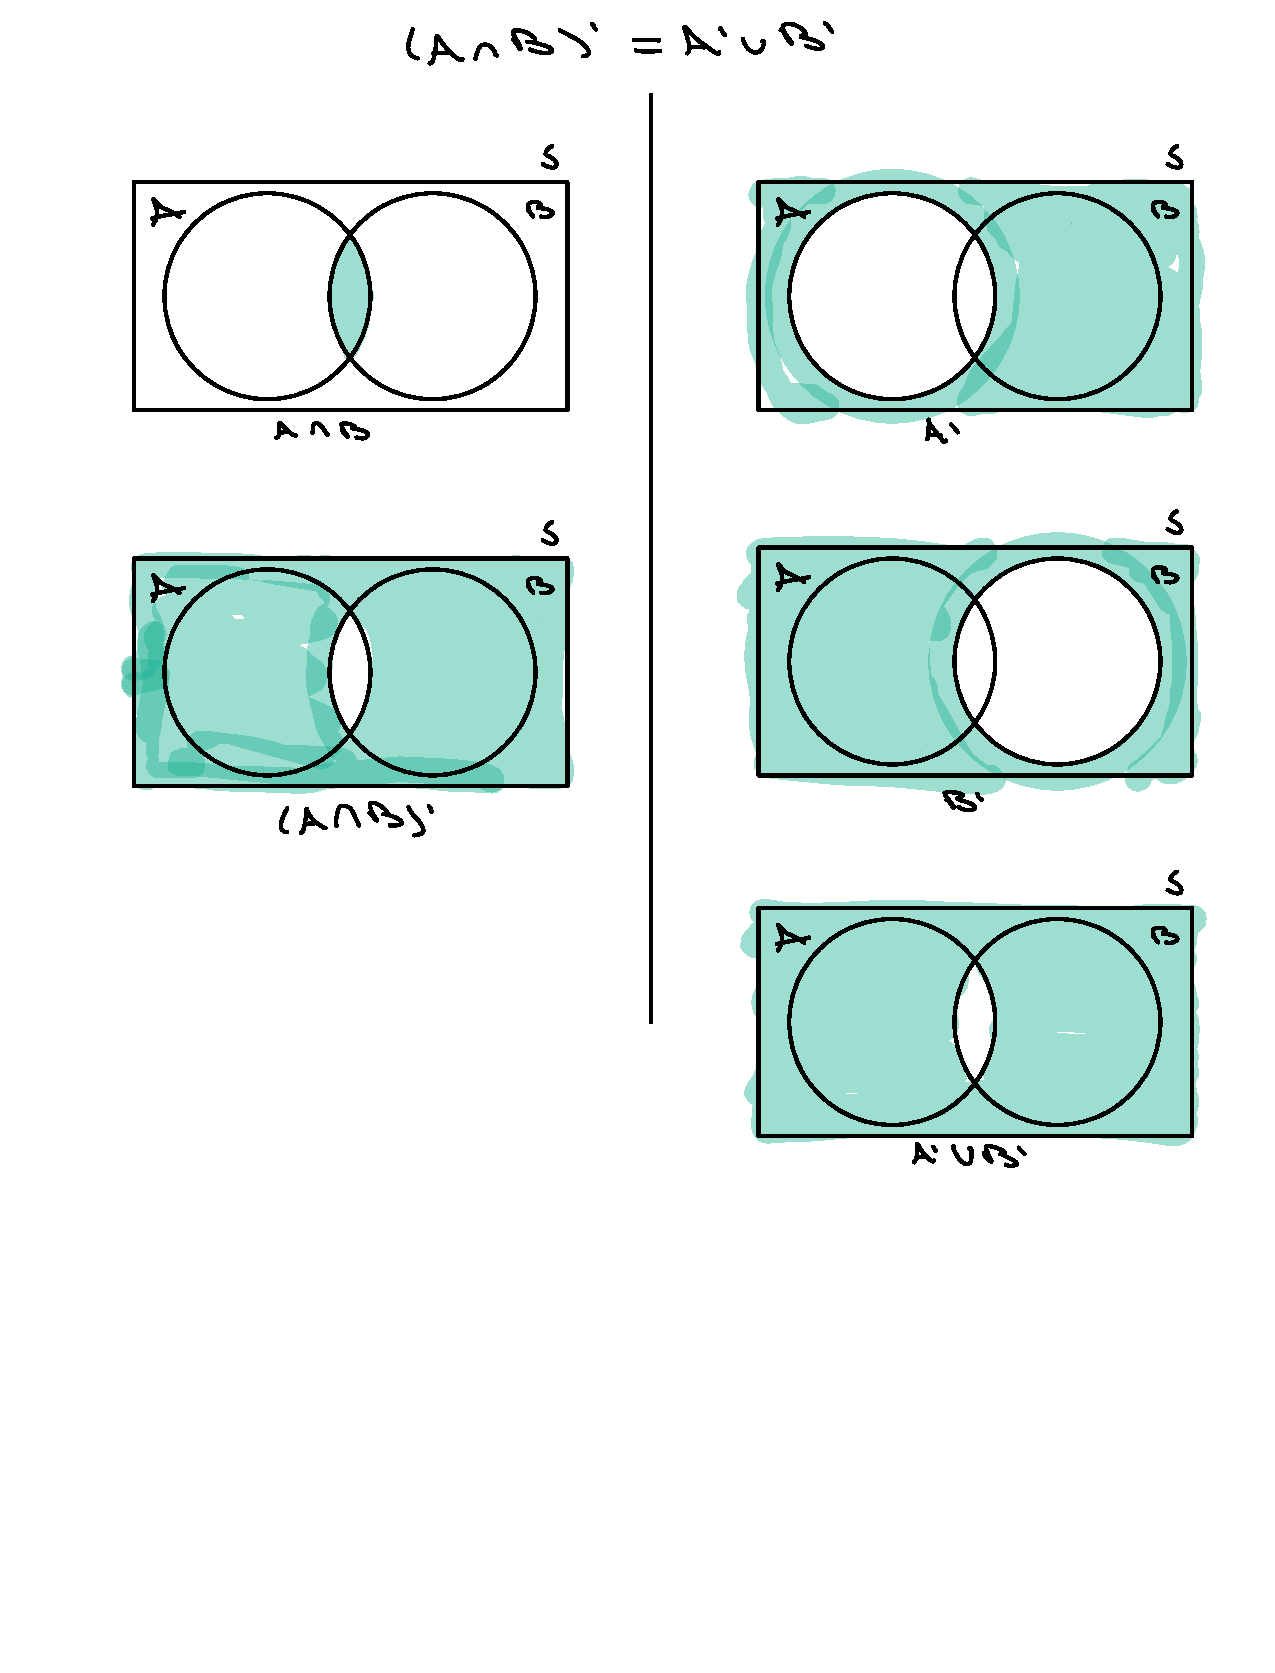
\includepdf[pages=-]{venn}

\end{document}
